\documentclass[11pt,a4paper]{article}

%\def\hidesols{hide solutions} % uncomment this line to hide solutions
\usepackage{../commons/course}


\شروع{نوشتار}

\سربرگ{تمرین سری اول}{لیست‌پیوندی، صف، پشته، درخت}{زمان آزمون: ۳ آذر}


 \مسئله{}
 
 نشان دهید یک صف را تنها با استفاده از دو پشته می‌توان طوری پیاده‌سازی کرد که هزینه سرشکن 	هر عمل enqueue و dequeue از $O(1)$   باشد.
 
 \مسئله{}
 
 یک quack داده‌ساختاری است که قابلیت صف و پشته را با هم دارد. در واقع آن را می‌توان به صورت یک لیست از اعضا که از چپ به راست نوشته شده‌اند، مشاهده کرد که سه عمل زیر را پشتیبانی می‌کند:\\
 \begin{itemize} 
 \item
Push یک عضو جدید به انتهای سمت چپ لیست اضافه می‌کند.
\item
Pop سمت چپ ترین عضو لیست را حذف می‌کند.
\item
Pull سمت راست ترین عضو لیست را حذف می‌کند.\\
\end{itemize}
 داده ساختار quack را با استفاده از 3  پشته و جافظه‌ی اضافی $O(1)$ طوری پیاده‌سازی کنید که زمان سرشکن هریک از این اعمال از $O(1)$ باشد. توجه کنید که تنها نوع دسترسی به هر کدام از این 3  پشته  از طریق اعمال push  و pop می‌باشد.
 
  \مسئله{}
  
  فرض کنید $n$  ورودی به یک پشته به ترتیب داده شده است. پشته در هر مرحله می‌تواند عمل push را انجام دهد و یک عنصر از ورودی بخواند و یا می‌تواند با عمل pop یک عنصر را در خروجی قرار دهد. در نهایت تمام  $n$  عنصر از ورودی وارد پشته شده و در خروجی قرار می‌گیرند و دنباله‌ی خروجی تولید می‌شود. تعداد دنباله‌های خروجی را که پشته می‌تواند تولید کند بیابید.
    
 \مسئله{}
 
 منظور از عمل getMin برگرداندن کوچکترین عنصر و getMax برگرداندن بزرگترین عنصر در داده‌ساختار است.
 
 \شروع{ابجد}
 \فقره داده‌ساختاری شبیه پشته ارائه دهید که اعمال Push و Pop و getMin  و getMax را در زمان سرشکن $O(1)$ انجام دهد.
 \فقره داده‌ساختاری شبیه صف ارائه دهید که اعمال enqueue و dequeue و getMin و getMax را در زمان سرشکن $O(1)$  انجام دهد.
 \پایان{ابجد}
 \مسئله{}
 
 یک لیست پیوندی از اعداد داریم که در آن هر عضو تنها به عضو بعدی دسترسی دارد. روشی کارا ارائه دهید که بدون تغییر در ساختار لیست و تنها با استفاده از $O(1)$ حافظه اضافی مشخص کند که آیا در این لیست دور وجود دارد  یا خیر. (توجه کنید که ساختار لیست در طول اجرای الگوریتم ثابت بماند و یکسان ماندن آن تنها در ابتدا و انتها کافی نیست) کارایی الگوریتم خود را ثابت کنید.


\مسئله{}

یک deque داده‌ساختاری مانند صف است با این تفاوت که عمل درج و حذف از هر دو طرف در آن صورت می‌گیرد. داده ساختار deque را با استفاده از یک آرایه پیاده‌سازی کنید بدین‌صورت که چهار رویه با زمان اجرای $O(1)$ بنویسید که اعمال درج و حذف عنصر از دو طرف را انجام دهند.


\مسئله{}

نشان دهید می‌توان با استفاده از یک آرایه و حافظه‌ی اضافی $O(1)$ دو پشته را پیاده‌سازی کرد. (توجه کنید که زمانی یک پشته نمی‌تواند عمل Push را انجام دهد که کل آرایه پر شده باشد)

\مسئله{}
\\
در یک گراف مرکز به رأسی گفته می شود که فاصله‌ی دورترین رأس از آن کمینه باشد. ثابت کنید مرکز یک درخت یا یک رأس است و یا دو رأسی که با یکدیگر همسایه‌اند.



\مسئله{}

پیش پردازشی از $O(n\log n)$ روی یک درخت ریشه‌دار اجرا کنید که بتوان پرسمان زیر را در $O(1)$ پاسخ داد: 
\\
آیا گره‌ی $u$ از اجداد گره‌ی $v$ هست یا خیر؟

\مسئله {}

درخت زیر را به شکل درخت چپ‌ترین فرزند-برادر راست تغییر دهید و سپس پیمایش میان‌ترتیب آن را به دست آورید. این پیمایش مشابه چه پیمایشی در درخت اصلی است؟ ادعای خود را در حالت کلی ثابت کنید.

\begin{figure}[h!]
\centering
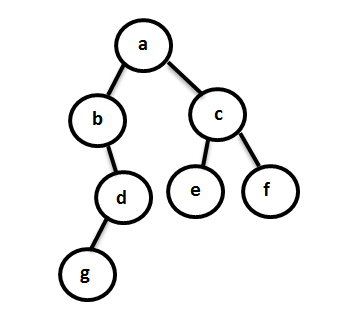
\includegraphics[scale=0.6]{pic7.png}
\label{overflow}
\end{figure}

\مسئله{}

هرم کمینه ای شامل $n$ عدد داریم. روشی ارائه دهید که بتواند به پرسش زیر در $O(i)$ پاسخ بدهد:
\\
آیا $i$ امین کوچکترین عدد از $x$ بزرگتر است یا خیر؟


\مسئله{}

برای عبارت
$((((a – b) * c) + d) – ((e / g) / h))$

\شروع{ابجد}
\فقره
درخت عبارت رسم کنید.
\فقره
پیمایش پیش‌ترتیب، میان‌ترتیب و پس‌ترتیب بنویسید.
\پایان{ابجد}

\مسئله{}

زبان $A$ از $n$ کلمه و زبان $B$ از $m$ کلمه تشکیل شده است. حروف به کار رفته در کلمات این دو زبان از مجموعه حروف الفبای فارسی است. بنابراین حداکثر ۳۲ حرف داریم. می‌دانیم طول هر کلمه در هر دوی این دو زبان حداکثر ۱۰۰ حرف است. می‌گوییم کلمه‌ی $w$ در زبان $X$ یافت می‌شود اگر و فقط اگر کلمه‌ای مانند $S$ در $X$ وجود داشته باشد که $w$ پیشوند $S$ باشد.


الگوریتمی از مرتبه‌ی $O(m + n)$ ارائه دهید که همه‌ی کلماتی از زبان $B$ را که در زبان $A$ یافت می‌شوند، چاپ کند.

\مسئله{}

ثابت کنید اگر $T(n)$ زمان پیمایش درخت دودویی با $n$ رأس باشد، برای هریک از پیمایش‌های پیش‌ترتیب، میان‌ترتیب و پس‌ترتیب ثابت کنید
$T(n) \in \Theta(n)$.

\مسئله{}

فرض کنید $T$ یک درخت دودویی کامل با $n$ گره و به ارتفاع $\log n$ است. می‌خواهیم مسیر ساده‌ای بین یک رأس $v$ به یک رأس $u$ پیدا کنیم. گره‌های $u$ و $v$ داده‌ شده‌اند و می‌دانیم که هر گره از این درخت به گره‌های فرزند و گره‌ی پدر دسترسی دارد. این کار را با چه مرتبه‌ای می‌توان انجام داد؟

\مسئله{}

درخت مبنا درختی دودویی است که مانند ترای، مجموعه‌ای از رشته‌های ساخته شده از ۰ و ۱ را نشان می‌دهد. در این درخت، هر گره متناظر با یک رشته است: برای ریشه این رشته تهی است. رشته‌ی هر گره برابر رشته‌ی پدر این گره به اضافه‌ی یک حرف است؛ این حرف برابر ۱ است اگر فرزند راست باشد و ۰ است اگر فرزند چپ باشد. هر گره علاوه بر اشاره‌گر به فرزندان راست و چپ حاوی یک متغیر منطقی است. اگر رشته‌ی متناظر با این گره در مجموعه‌ی رشته‌های درخت مبنا وجود داشته باشد، این متغیر ۱ است.

\شروع{ابجد}
\فقره
رشته‌های ۱۱۰۱، ۰۱۰۰، ۰۰۱۱، ۰۰۱۰، ۰۰۰۱، ۱۰۰۰ و ۱۰۰۱ را به ترتیب در یک درخت مبنای تهی درج می‌کنیم. درخت حاصل را رسم کنید.

\فقره
الگوریتمی طراحی کنید که با گرفتن مجموعه‌ای از $n$ رشته از ۰ و ۱، درخت مبنا را بسازد.
\پایان{ابجد}

\مسئله{}

یک درخت دودویی $T=(V,E)$ به ما داده شده (به شکل ماتریس مجاورت) و رأس پدر آن را نیز داریم. همچنین یک آرایه‌ی $x$ نیز داریم که به هر گره‌ی درخت یک عدد نسبت می‌دهد. آرایه‌ی جدید $z$ را این‌گونه بسازید که برای هر $u\in V$، $z[u]$ برابر ماکسیمم مقادیر $x$ برای نوادگان $u$ (\lr{descendants}) است. الگوریتمی خطی ($O(n)$) ارائه دهید تا آرایه‌ی $z$ را تماماً حساب کند.

\پایان{نوشتار}
